\documentclass[notheorems,mathserif,table,compress]{beamer}  %dvipdfm选项是关键,否则编译统统通不过
%%------------------------常用宏包------------------------
%%注意, beamer 会默认使用下列宏包: amsthm, graphicx, hyperref, color, xcolor, 等等
\usepackage{fontspec,xunicode,xltxtra}  % for XeTeX
\usepackage{comment}
\usepackage{fancybox}
 \usepackage{enumerate}
\usepackage{color}

%%------------------------ThemeColorFont------------------------
%% Presentation Themes
% \usetheme[<options>]{<name list>}
\usetheme{Madrid}
%% Inner Themes
% \useinnertheme[<options>]{<name>}
%% Outer Themes
% \useoutertheme[<options>]{<name>}
\useoutertheme{miniframes} 
%% Color Themes 
% \usecolortheme[<options>]{<name list>}
%% Font Themes
% \usefonttheme[<options>]{<name>}
\setbeamertemplate{background canvas}[vertical shading][bottom=white,top=structure.fg!7] %%背景色, 上25%的蓝, 过渡到下白.
\setbeamertemplate{theorems}[numbered]
\setbeamertemplate{navigation symbols}{}   %% 去掉页面下方默认的导航条.
\usepackage{zhfontcfg}
\usepackage{wrapfig}
%\setsansfont[Mapping=tex-text]{文泉驿正黑}  %% 需要fontspec宏包
     %如果装了Adobe Acrobat,可在font.conf中配置Adobe字体的路径以使用其中文字体
     %也可直接使用系统中的中文字体如SimSun,SimHei,微软雅黑 等
     %原来beamer用的字体是sans family;注意Mapping的大小写,不能写错
     %设置字体时也可以直接用字体名,以下三种方式等同:
     %\setromanfont[BoldFont={黑体}]{宋体}
     %\setromanfont[BoldFont={SimHei}]{SimSun}
     %\setromanfont[BoldFont={"[simhei.ttf]"}]{"[simsun.ttc]"}
%%------------------------MISC------------------------
\graphicspath{{figures/}}         %% 图片路径. 本文的图片都放在这个文件夹里了.
%%------------------------正文------------------------
\begin{document}
\XeTeXlinebreaklocale "zh"         % 表示用中文的断行
\XeTeXlinebreakskip = 0pt plus 1pt % 多一点调整的空间
%%----------------------------------------------------------
%% This is only inserted into the PDF information catalog. Can be left
%% out.
%%%
%% Delete this, if you do not want the table of contents to pop up at
%% the beginning of each subsection:
\begin{comment}
\AtBeginSection[]{                              % 在每个Section前都会加入的Frame
  \frame<handout:0>{
    \frametitle{Content}\small
    \tableofcontents[current,currentsubsection]
  }
}
\AtBeginSubsection[]                            % 在每个子段落之前
{
  \frame<handout:0>                             % handout:0 表示只在手稿中出现
  {
    \frametitle{下一节内容}\small
    \tableofcontents[current,currentsubsection] % 显示在目录中加亮的当前章节
  }
}
\end{comment}
%%----------------------------------------------------------
\title[Graph-based Segmentation]{Graph-based Segmentation}
\subtitle{基于图论的图像分割}
\author[戴嘉伦\ 王如晨\  赵海伟]{\textcolor{olive}{ 戴嘉伦\ 王如晨\ 赵海伟 }}
  %\hspace{2.28em}导师~~\textcolor{olive}{姬光荣}~教授}
\institute[CVBIOUC]{\small\textcolor{violet}{CVBIOUC}}
\date{\today}
%\titlegraphic{\vspace{-6em}\includegraphics[height=7cm]{ouc}\vspace{-6em}}
\frame{ \titlepage }
%%----------------------------------------------------------
%\section*{目录}
\frame{\frametitle{目录}\tableofcontents}
%%----------------------------------------------------------

%\section{Beamer类和XeTeX概览} %如果你想书签不出现问题,请不要用\XeTeX
                                 %这类复杂的指令,直接写XeTeX吧
\begin{comment}
\section{Graph}
\begin{frame}
\frametitle{Graph}
    \begin{figure}[!ht]
     \centering
     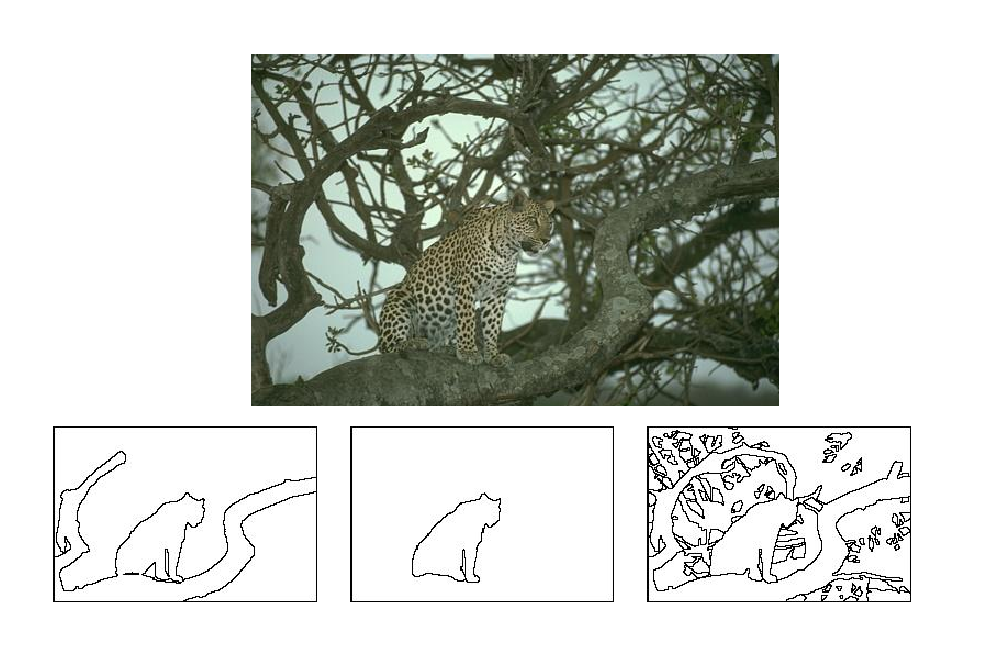
\includegraphics[width=2.5in]{pic.png} \\
     \end{figure}
\end{frame}
\end{comment}

\section{Graph}
\begin{frame}
    \frametitle{Graph}
    \begin{columns}
       \begin{column}[c]{0.5\textwidth}
          {\textbf{\Large Graph}}:\\
          \begin{itemize}
	  \item[-] node
	  \item[-] link
	  \item[-] weight
	  \item[-] direction
          \end{itemize}
      \end{column}
  
      \begin{column}[c]{0.5\textwidth}
          \begin{figure}[!ht]
          \centering
          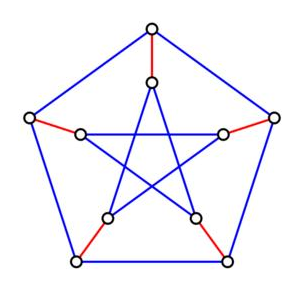
\includegraphics[width=1.3in]{GRAPH.png}
          \end{figure}
     \end{column}
   \end{columns}
%A graph is a set of nodes V and edges E that connect vaxerious nodes; G={V, E}\\
%A weighted graph is the one in which weight is associated with each edge\\
%A connected graph is the one where every pair of nodes is connected.
\end{frame}


\begin{frame}
    \frametitle{Graph}
    \begin{columns}
       \begin{column}[c]{0.5\textwidth}
          {\textbf{\Large Image as graph}}:\\
          \begin{itemize}
	  \item[-] {\color{blue} node} for every pixel
	  \item[-] {\color{blue} link} between every pair of pixels
	  \item[-] {\color{blue} weight} of link for similarity 
          \end{itemize}
      \end{column}
  
      \begin{column}[c]{0.5\textwidth}
          \begin{figure}[!ht]
          \centering
          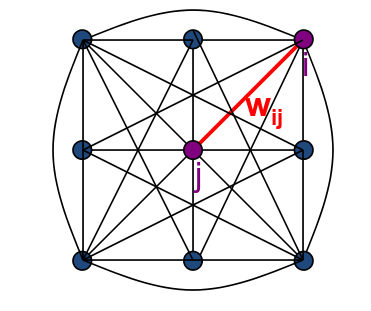
\includegraphics[width=1.6in]{image.png}
          \end{figure}
     \end{column}
   \end{columns}
%A graph is a set of nodes V and edges E that connect vaxerious nodes; G={V, E}\\
%A weighted graph is the one in which weight is associated with each edge\\
%A connected graph is the one where every pair of nodes is connected.
\end{frame}

\begin{frame}
   \frametitle{Graph}
    \begin{columns}
       \begin{column}[c]{0.45\textwidth}
          \begin{figure}[!ht]
          \centering
          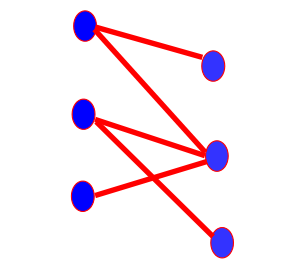
\includegraphics[width=1.0in]{G_VE.png}\\
	  {\textbf{\huge $G=(V,E)$}}
          \end{figure}
         \hspace{0.3in} $V$ $(Vertex)$: Nodes \\
	  \hspace{0.3in} $E$ $(Edge)$: Links
       %% A graph $G=(V,E)$ is a triple consisting of a vertex set $V(G)$, an edge set $E(G)$ and a  relation  that associates with each edge two vertices.\\
       %A graph $G$ is connected if there is a path from every vertex to every other vertex in $G$.
       \end{column}

       \begin{column}[c]{0.55\textwidth}
          \begin{figure}[l]
          \centering
          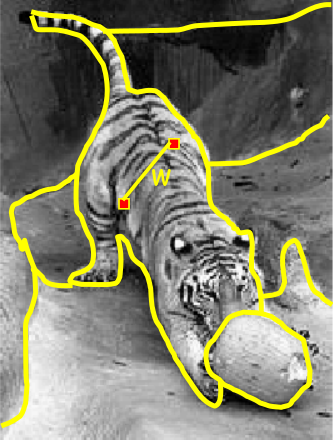
\includegraphics[width=0.9in]{G_VE1.png}
          \end{figure}
      \hspace{0.4in} Image = \{ pixels\} \\
     \hspace{0.4in}  Pixel similarity
      \end{column}
    \end{columns}
\end{frame}

\begin{comment}
\begin{frame}
   \frametitle{Graph}
    A graph $G={V,E}$ is a triple consisting of a vertex set $V(G)$, an edge set $E(G)$ and a relation that associates with each edge two vertices.\\
    A graph $G$ is connected if there is a path from every vertex to every other vertex in $G$.\\
    The weight of edges means the similarity of two connecting pixels.\\
    The bigger the weight is, the more similar two pixels are.  
    \begin{figure}[!ht]
    \centering
    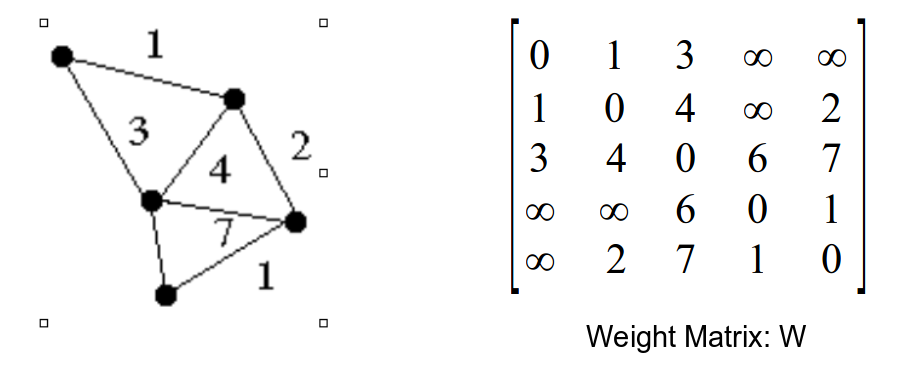
\includegraphics[width=3.0in]{graph2}
    \end{figure}
\end{frame}
\end{comment}

\begin{frame}
\frametitle{Graph}
    \begin{figure}[!ht]
     \centering
     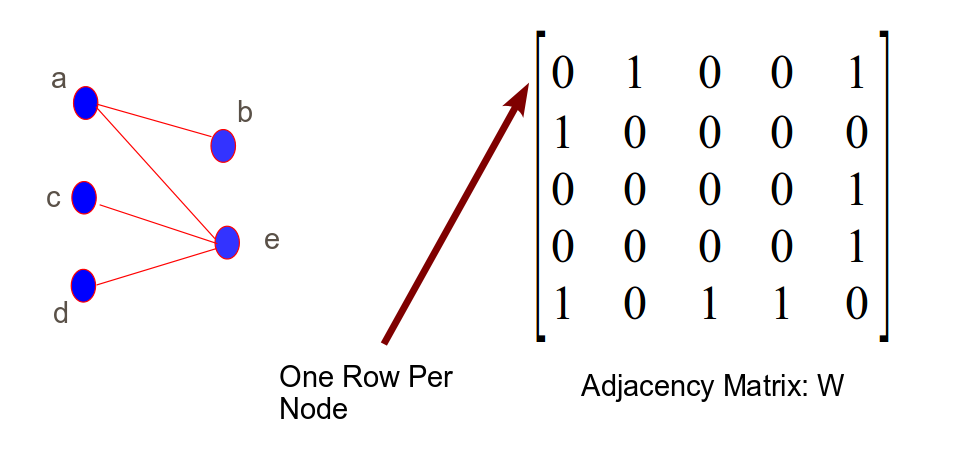
\includegraphics[width=2.5in]{graph.png} \\
      A graph can be represented with a matirx.
     \end{figure}
\end{frame}

\begin{frame}
   \frametitle{Graph}
   \begin{columns}
     \begin{column}[c]{0.4\textwidth}
	\textbf{\Large Cut}:
	\begin{itemize}
	\item[-] {\color{blue} sub-set} of edges $E$
	\item[-] set of links whose removal makes a graph {\color{blue} disconnected}
	\item[-] {\color{blue} cost} of partition\newline
	\end{itemize}
\begin{displaymath}
Cut(A,B)= \sum_{i\in A, j\in B} w(i,j)
\end{displaymath} %such that removal of $S$ from $G$ disconnects $G$.
    \end{column}

    \begin{column}[c]{0.6\textwidth}
    \centering
    \begin{figure}[!ht]
    \centering
    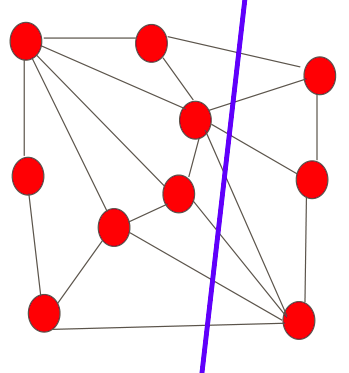
\includegraphics[width=1.2in]{graph3.png}
    \end{figure}
    \begin{figure}[!ht]
    \centering
    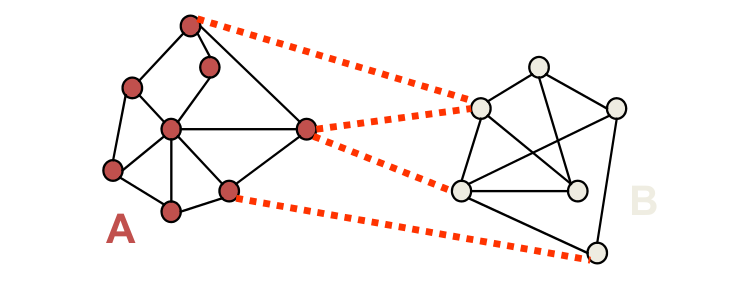
\includegraphics[width=2.4in]{graph_based.png}
    \end{figure}
    \end{column}
    \end{columns}
\end{frame}

\begin{frame}
\frametitle{Graph}

\textbf{\Large Weight}:
\begin{itemize}
\item[-] relation of pixels, $w(i,j)$
	\begin{itemize}
	\item[-] similarity
	\item[-] closeness\newline
	\end{itemize}
\end{itemize}
%So, the weight function definites the similarity of two nodes.
\begin{displaymath}
w_{ij}= \exp(\frac{{\parallel F_{i}-F_{j}\parallel}_{2}^2}{{\sigma}^2}) \times \left \{ \begin{array}{ll}
   \exp(\frac{{\parallel X_{i}-X_{j}\parallel}_{2}^2}{{\sigma}^2}) & \frac{{\parallel X_{i}-X_{j}\parallel}_{2}^2}{{\sigma}^2} < R\\
   \hspace{0.4in} 0 & \textrm{otherwise} 
    \end{array} \right.
\end{displaymath}
       \begin{itemize}
	\item[-]
	\begin{itemize}
	\item[-] value of gray scale $F_{i}$
	\item[-] position $X_{i}$ 
	\item[-] distance $R$
	\end{itemize}
      \end{itemize}
%$F_{i}$ means the value of gray scale, $X_{i}$ means the position, $r$ means the distance.\\
%Therefore, the similarity is determined by the value of gray scale and the distance of points.
\end{frame}

\begin{frame}
    \frametitle{Graph}
   \textbf{\Large Min Cut}:
\begin{itemize}
	\item[-] Minimum cut is the cut of minimum weight, where the value of $Cut(A,B)$ is minimum.\newline
\end{itemize}
    %Find some lowest weights of edges from vertex sets. It means that These points is not similar, and those not cut can be seen as one cluster. \\
    \begin{figure}
	\begin{minipage}[c]{0.4\textwidth}
	\centering
	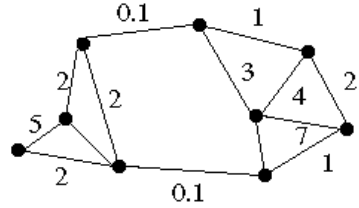
\includegraphics[width=1.5in]{mincut1}
	\end{minipage}
	\begin{minipage}[c]{0.4\textwidth}
	\centering
	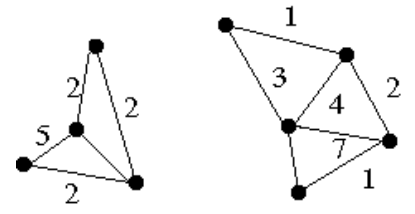
\includegraphics[width=1.7in]{mincut2}
	\end{minipage}
    \end{figure}
\end{frame}
   
\begin{frame}
    \frametitle{Graph}
    \textbf{\Large Min Cut Problem}:\\
        \begin{itemize}
	\item Min Cut will choose a cut with one small cluster.
%	\item The Min Cut favors cuttingsmall sets of isolated nodes in the graph.
	\end{itemize}
    \begin{figure}[!ht]
    \centering
    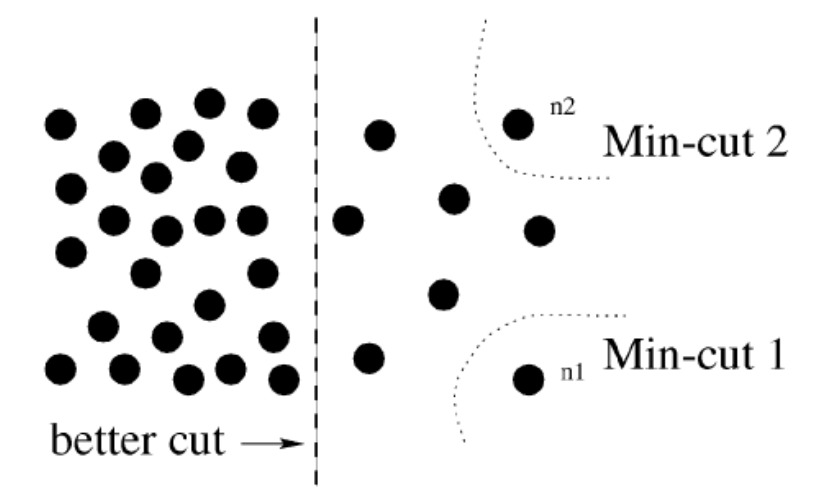
\includegraphics[width=2.5in]{min_cut}
    \end{figure}
\end{frame}


%\begin{frame}
%\frametitle{Min Cut Problem}Some points which are far away from most points  may be partitioned into one cluster.
%\end{frame}

\section{Normalized Cuts}
\begin{frame}
\frametitle{Normalized Cuts}
   \textbf{\Large Normalized Cuts\footnote{``Normalized Cuts and Image Segmentation'', JianBo Shi and Jitendra Malik. PAMI, 2000}}:\\
   \begin{itemize}
   \item[-] {\color{blue} cut} is minimum 
   \item[-] {\color{blue} cluster} size is similar
   \end{itemize}
\end{frame}


\begin{frame}
\frametitle{Normalized Cuts}
   \textbf{\Large NCut}:\\
\begin{displaymath}
NCut(A,B)= \frac{Cut(A,B)}{assoc(A,V)} + \frac{Cut(A,B)}{assoc(B,V)}	
\end{displaymath}

\begin{itemize}
\item[-] 
\end{itemize}

\begin{itemize}
\item[-] $Cut(A,B) $: the {\color{blue} cost} of partition as $A$ and $B$ 
\end{itemize}
\[ Cut(A,B) = \sum_{i\in A, j\in B} w(i,j) \]
\begin{itemize}
\item[-] $assoc(A,V)$: {\color{blue} volume} of set $A$. 
\end{itemize}
\[ asscoc(A,V)=\sum_{i \in A} {d_{i}} \]
\[ d_{i} = { \sum_{j \in V} w(i,j)} \]
%\begin{itemize}
%\item[-] $assoc(B,V) $
%\end{itemize}
\end{frame}




\begin{frame}
\frametitle{Normalized Cuts}
\begin{flalign*}
NCut(A,B)&= \frac{Cut(A,B)}{assoc(A,V)} + \frac{Cut(A,B)}{assoc(B,V)}	&\\
	 &= {\frac{\sum_{(x_{i}>0,x_{j}<0)} {-w_{ij}} \cdot x_{i} \cdot x_{j} }{\sum_{x_{i}>0} d_{i}}} + {\frac{\sum_{(x_{i}>0,x_{j}<0)} {-w_{ij}} \cdot x_{i} \cdot x_{j} }{\sum_{x_{j}<0} d_{i}}}& \\
\end{flalign*}
%If x $\in$ A, x=1; else x=-1\\
\begin{displaymath}
 y=(1+x)-b(1-x) 
\end{displaymath} 
\begin{displaymath}
 \min_{x} NCut(x)=\min_{y} \frac{y^T (D-W) y}{y^T D y} 
\end{displaymath}
\begin{displaymath}
 \Longrightarrow (D-W) y = \lambda D y 
\end{displaymath} 
\end{frame}



\begin{frame}
\frametitle{Normalized Cuts}
\textbf{\Large Recursive normalized cuts}:
\begin{itemize}
\item[-] Given an image or image sequence, set up a {\color{blue} weighted graph}: $ G=(V,E) $
	\begin{itemize}
	\item[-] Vertex for each pixel
	\item[-] Edge weight for nearby pairs of pixels
	\end{itemize}
\item[-] Solve for {\color{blue} eigenvecotrs} with the smallest eigenvalues: $ (D-W)y=\lambda Dy $
	\begin{itemize}
	\item[-] Use the eigenvector with the second smallest eigenvalue to bipartition the graph
	\item[-] The result is an approximation
	\end{itemize}
\item[-] Recursively repartition the segmented parts if necessary
\end{itemize}
\end{frame}

\begin{comment}
\begin{frame}
\frametitle{Normalized Cut}
If x $\in$ A, x=1; else x=-1\\
\begin{displaymath}
\min_{x} NCut(x)=\min_{y} \frac{y^T (D-W) y}{y^T D y} 
\end{displaymath} 
\begin{displaymath}
(D-W) y = \lambda D y
\end{displaymath} 
\end{frame}
\end{comment}

\begin{frame}
\frametitle{Normalized Cuts}
\textbf{\Large Adavantage}:
\begin{itemize}
\item[-] Generic framework that can be used with different features and affinity formulations
\item[-] Provides regular segments \\
\end{itemize}
\textbf{\Large Disadavantage}:
\begin{itemize}
\item[-] Need to chose number of segments
\item[-] High sotrage requirement and time complexity
\item[-] Bias towards partitioning into equal segments
\end{itemize}
\end{frame}


\begin{frame}
\frametitle{Normalized Cuts}
    \hspace{0.5in} {\color{blue} [Demo]}
    \begin{figure}[!ht]
     \centering
     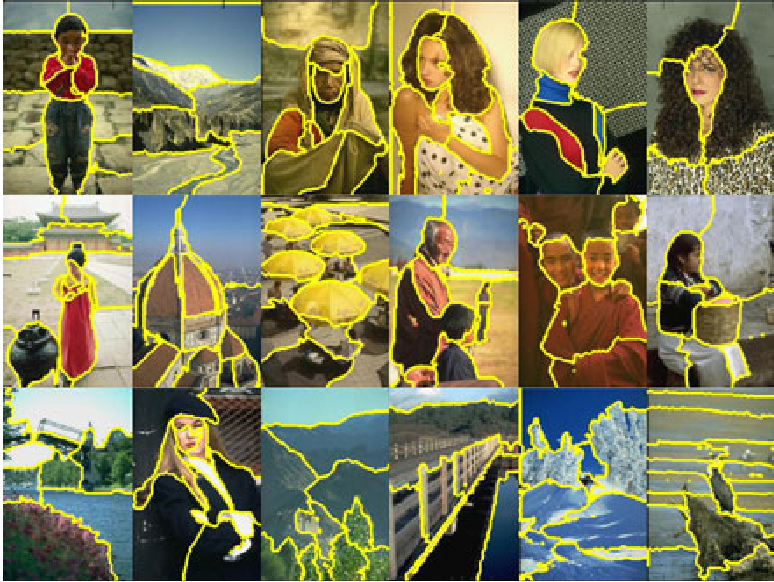
\includegraphics[width=2.5in]{NORMALE.png} 
     \end{figure}
\end{frame}

\section{Graph Cuts}
\begin{frame}
\frametitle{Graph Cut}
  \begin{figure}[!ht]
  \centering
   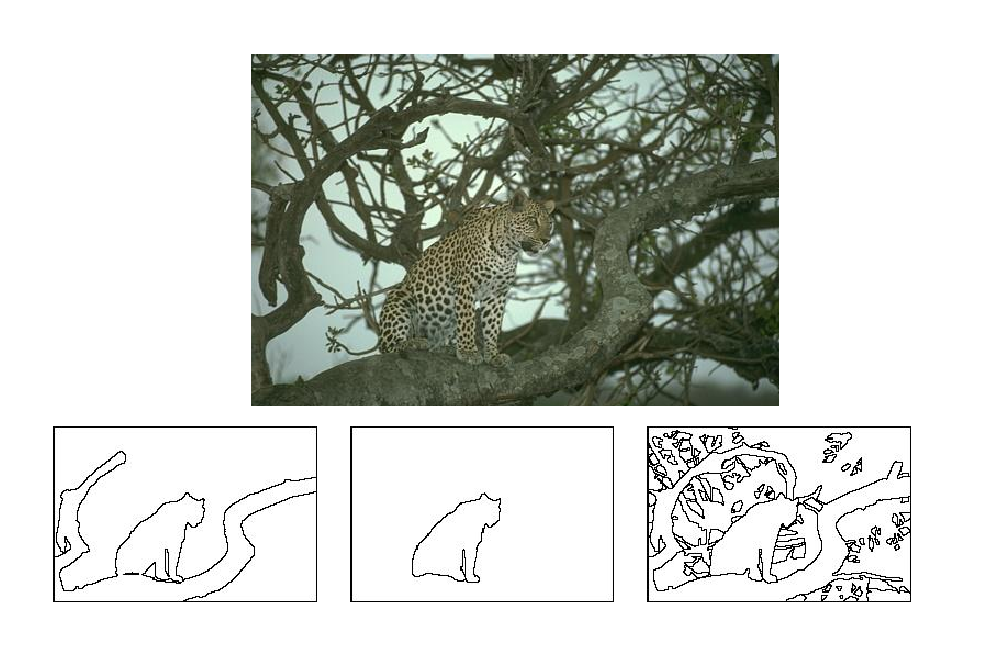
\includegraphics[width=3.4in]{pic.png}
   \end{figure}
\end{frame}


\begin{frame}
\frametitle{Graph Cuts\footnote{``Interactive Graph Cuts for Optimal Boundary \& Region Segmentation of Objects in N-D Images'', Boykov. ICCV, 2001}}
%\textbf{\Large Graph Cut}:
\begin{itemize}
\item[-] Two kinds of {\color{blue} vertices} 
	\begin{itemize}
	\item[-] {\color{blue} normal} vertices : nodes
	\item[-] {\color{blue} terminal} vertices: S (source point), T (sink point)
	\end{itemize}
\item[-] Two kinds of {\color{blue} edges}
	\begin{itemize}
	\item[-] {\color{blue} n-link}: node to node
	\item[-] {\color{blue} t-link}: s-node or t-node to node
	\end{itemize}
\end{itemize}
%new terminal vertex $"S"$,$"T"$ are added to the vertex $V$, so the edge can be divided as n-links and t-links\\
%s $\rightarrow$ 前景 \\
%s $\rightarrow$ 背景 
\begin{figure}[!ht]
    \centering
    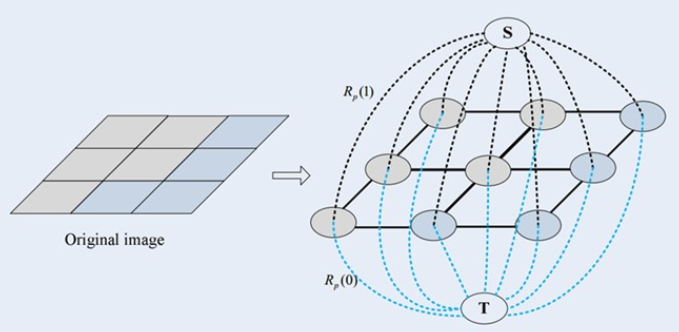
\includegraphics[width=2.8in]{graph_cut}
\end{figure}
\end{frame}




\begin{frame}
\frametitle{Graph Cuts}
    \begin{figure}[!ht]
    \begin{minipage}[t]{0.45\linewidth}
    \centering
    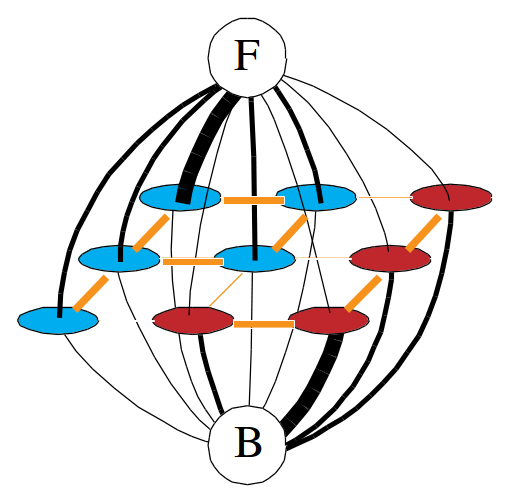
\includegraphics[width=1.0in]{graphcut1.png}
    \end{minipage}
    \begin{minipage}[t]{0.45\linewidth}
    \centering
    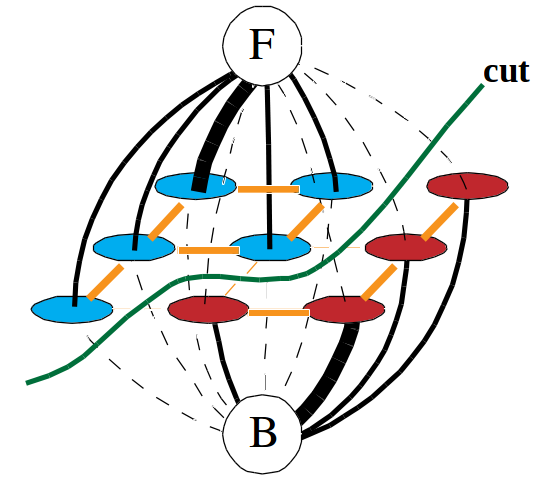
\includegraphics[width=1.1in]{graphcut2.png}
    \end{minipage}
    \end{figure}

    \begin{columns}
       \begin{column}[c]{0.4\textwidth}
	
%	  {\textbf{Label image with ${0,1}$}}
%	  \begin{itemize}
%	  \item[-] ``foreground'' pixel is 1
%	  \item[-] ``background'' pixel is 0 \\
%	  \end{itemize}
	  \begin{itemize}
	\centering
	  \item[-]  {\Large S $\Rightarrow$ foreground}
	  \item[-] {\Large T $\Rightarrow$ background }
	  \item[-] {\Large  S $\cup$ T = V}
	  \end{itemize}
        \end{column}
 
      \begin{column}[c]{0.6\textwidth}
          \begin{figure}[!ht]
          \centering
          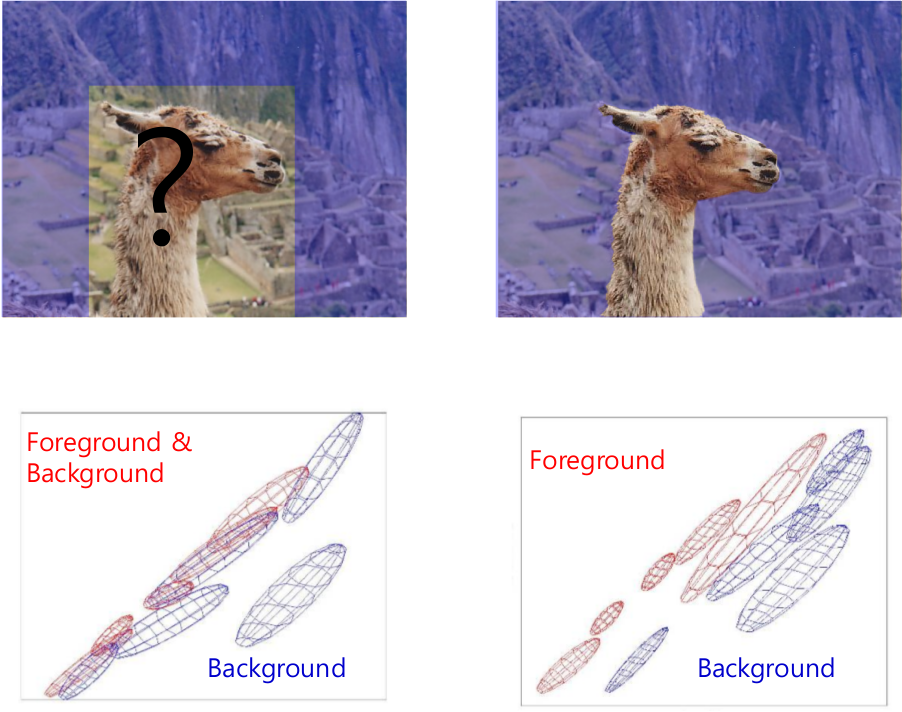
\includegraphics[width=1.9in]{GRAB2.png}
          \end{figure}
 %         \begin{figure}[!ht]
 %         \centering
 %         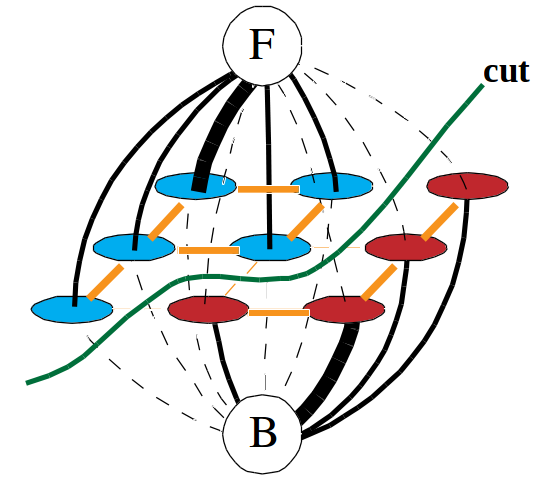
\includegraphics[width=1.2in]{graphcut2.png}
 %         \end{figure}
      \end{column}
   \end{columns}
%$A=(A_{1},A_{2},\cdots A_{P})$ means a binary vector, $P$ means the numbers of pixels, $A_{P}$ means the label of $P$ pixel
%\begin{displaymath}
%E(A) = \lambda R(A) + B(A)
% \end{displaymath} 
\end{frame}


\begin{comment}
\begin{frame}
%\begin{displaymath}
\hspace{0.3in}$R(A) = \sum_{p \in P} {R_{p} (A_{p})}$
%\end{displaymath}
\begin{itemize}
\item[-] ``foreground'' pixel is 1
\item[-] ``background'' pixel is 0 \\
\end{itemize}
\begin{displaymath}
B(A)=\sum_{p,q \in N} {B(p,q) \delta (A_{p}, A_{q})}, \hspace{0.2in}
\delta (A_{p}, A_{q})= \left \{ \begin{array}{ll}
  = 1 & A_{p} \neq A_{q}\\
    0 & \textrm{otherwise} 
    \end{array} \right.
\end{displaymath}
\end{frame}




\begin{frame}
\frametitle{Graph Cut}
binary label in image, the pixel in 前景 is 1, background is 0 \\
$A=(A_{1},A_{2},\cdots A_{P})$ means a binary vector, $P$ means the numbers of pixels, $A_{P}$ means the label of $P$ pixel
\begin{displaymath}
E(A) = \lambda R(A) + B(A)
\end{displaymath} 
%\begin{displaymath}
\hspace{0.3in}$R(A) = \sum_{p \in P} {R_{p} (A_{p})}$
%\end{displaymath}
\begin{displaymath}
B(A)=\sum_{p,q \in N} {B(p,q) \delta (A_{p}, A_{q})}, \hspace{0.2in}
\delta (A_{p}, A_{q})= \left \{ \begin{array}{ll}
  = 1 & A_{p} \neq A_{q}\\
    0 & \textrm{otherwise} 
    \end{array} \right.
\end{displaymath}
\end{frame}
\end{comment}

\begin{frame}
\frametitle{Graph Cuts}
	  {\textbf{Label image with ${0,1}$}}
	  \begin{itemize}
	  \item[-] ``object'' pixel is 1
	  \item[-] ``background'' pixel is 0 \\
	  \end{itemize}

{\textbf{Data element set $P$ representing the image pixels}}
\begin{itemize}
\item[-] $A=(A_{1},A_{2},\cdots, A_{p},\cdots, A_{P})$,	\hspace{0.1in} $A_{p}=\{ 0, 1 \}$
	\begin{itemize}
	\item[-] $P$ the number of pixels
	%\item[-] Neighborhood system as a set $N$ representing all pairs $\{ p,q \}$ of neighboring elements in $P$
	\item[-] $A_{p}$ the label of pixel $p$
	\end{itemize}
\end{itemize}
\end{frame}


\begin{frame}
\frametitle{Graph Cuts}
\textbf{Energy Function}:
\begin{flalign*} 
 E(A) &=\lambda \cdot R(A) + B(A) & \\
      &=\lambda \cdot \sum_{p \in P} R_{p}(A_{p}) + \sum_{p \in P} \sum_{\{ p,q\} \in N} B_{\{ p,q\}} \cdot  \delta (A_{p}, A_{q}) &
%& R(A)=\sum_{p \in P} R_{p}(A_{p}) &\\
%& B(A)=\sum_{p \in P} \sum_{\{ p,q\} \in N} B_{\{ p,q\}} \cdot  \delta (A_{p}, A_{q}) &\\
%& \delta (A_{p}, A_{q}) = \left \{ \begin{array}{ll}
%  1 & {A_{p} \ne A_{q}}\\
%    0 & \textrm{otherwise}
%    \end{array} \right. &
\end{flalign*}

\begin{itemize}
\item[-] $R(A)$ defines {\color{blue} penalties} for assigning each pixel to object or background %, which are $R_{p}$(``obj'') and $R_{p}$ (``bkg'')
	\begin{itemize}
	\item[-] \textbf{t-link}
	\item[-] $R_{p}$(``obj'') is lower, \hspace{0.1in} $p$ belongs to object 
	\item[-] $R_{p}$(``bkg'') is lower, \hspace{0.1in} $p$ belongs to background
	\end{itemize}
\item[-] $B(A)$ sets {\color{blue} penalties} of discontinuities between pixels
%, $B_{\{p,q\}}$ is large when $p$ and $p$ are similar, it is close to 0 when $p$ and $p$ are very different
	\begin{itemize}
	\item[-] \textbf{n-link}
	\item[-] $B(A)$ describes the boundary properties of the segmentation
	\item[-] $B_{\{p,q\}}$ is large, \hspace{0.1in} $p$ and $q$ are similar
	\item[-] $B_{\{p,q\}}$ $\rightarrow$ 0, \hspace{0.1in} $p$ and $q$ are different
	\end{itemize}
\end{itemize}
\end{frame}


\begin{frame}
\frametitle{Graph Cuts}
  \begin{figure}[!ht]
  \centering
   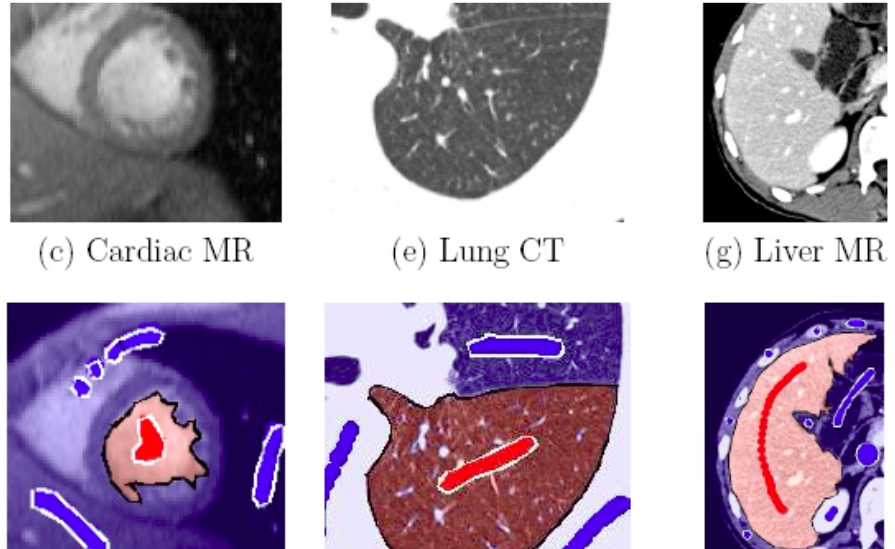
\includegraphics[width=2.5in]{graphcut4.png}
   \end{figure}
\end{frame}



\begin{frame}
\frametitle{Graph Cuts}
  \begin{figure}[!ht]
  \centering
   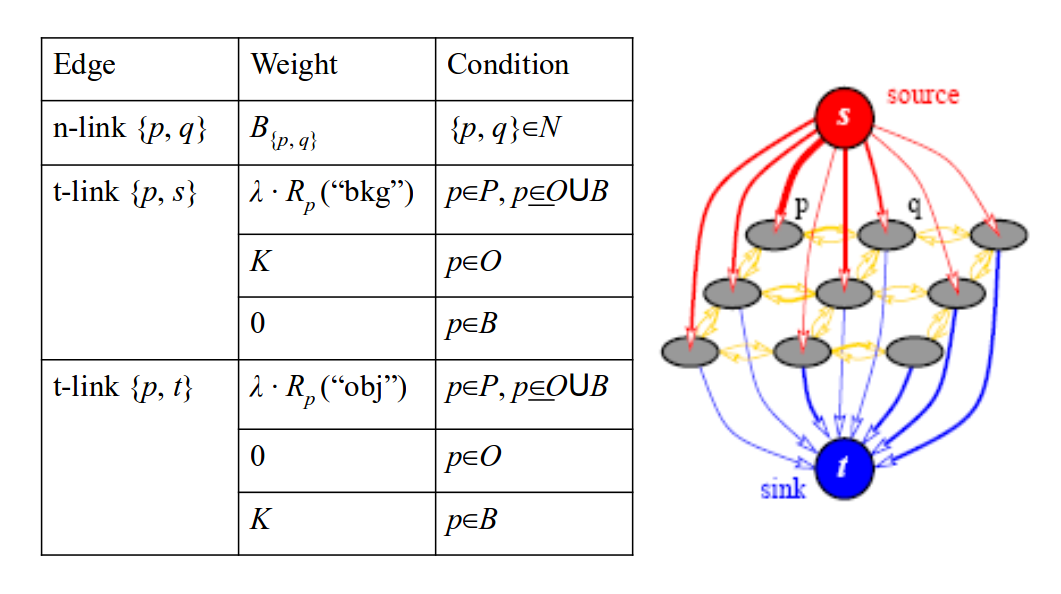
\includegraphics[width=2.5in]{graphcut3.png}
   \end{figure}
\end{frame}

\begin{comment}
\begin{frame}
\begin{flalign*} & R(f)=\sum_{p\in S} {D_{p}(f_p)} & \end{flalign*}
\begin{itemize}
\item[-] Region 
\item[-] $D_{p}(f_{p})$ is the cost of piexel labeled as $f_{p}$
\end{itemize}
 means region properties, $D_{p}(f_{p})$ is the cost of piexel labeled as $f_{p}$\\
Set pre-defined point as the sample of object and background, estimate the histogram of object and background as
$D_{p}("obj")=-\ln P_{r} (I_{p} \mid "obj"))$ and $D_{p}("bkg")=-\ln P_{r} (I_{p} \mid "bkg"))$
\end{frame}
\end{comment}


\begin{frame}
\frametitle{Graph Cuts}
\textbf{\Large t-links}: \begin{flalign*} & R(A)=\sum_{p\in P} {R_{p}(A_p)} & \end{flalign*}
\begin{itemize}
\item[-] Estimate {\color{blue}object and background} intensity distribution based on object or background seeds
\item[-] $R_{p}(obj)=-\ln P_{r}(A_{p} \mid obj)$
\item[-] $R_{p}(bkg)=-\ln P_{r}(A_{p} \mid bkg)$ \\
\end{itemize}
\begin{itemize}
\item[-]
	\begin{itemize}
	\item[-] \emph{if} $P_{r}(A_{p} \mid obj)$ $>$ $P_{r}(A_{p} \mid bkg)$
	    \begin{itemize}
		\item[-]  $R_{p}(obj)$ < $R_{p}(bkg)$
		\item[-]  the pixel belongs to object
	    \end{itemize}
	\item[-] \emph{else} 
	    \begin{itemize}
		\item[-]  $R_{p}(obj)$ >  $R_{p}(bkg)$
		\item[-]  the pixel belongs to background
	    \end{itemize}
	\end{itemize}
\end{itemize}
\end{frame}




\begin{frame}
\frametitle{Graph Cuts}
  \begin{figure}[!ht]
  \centering
   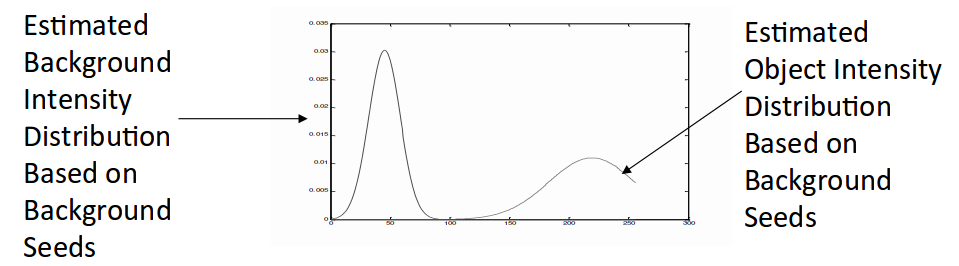
\includegraphics[width=4.0in]{t_link.png}
   \end{figure}
\end{frame}

\begin{comment}
\begin{frame}
\frametitle{Graph Cut}
$f_p$ means the label of pixel $p$ 对图像像素的标记就是从$V$ 到 $L$的映射, $f={f_{p} \mid f_{p} \in L}$\\
$E(f)=R(f)+\lambda B(f)$\\
$R(f)=\sum_{p\in S} {D_{p}(f_p)}$ means region properties, $D_{p}(f_{p})$ is the cost of piexel labeled as $f_{p}$\\
Set pre-defined point as the sample of object and background, estimate the histogram of object and background as
$D_{p}("obj")=-\ln P_{r} (I_{p} \mid "obj"))$ and $D_{p}("bkg")=-\ln P_{r} (I_{p} \mid "bkg"))$
\end{frame}
\end{comment}


\begin{frame}
\frametitle{Graph Cuts}
\textbf{\Large n-links}: 
\begin{flalign*} 
& B(A)=\sum_{p \in P} \sum_{\{ p,q\} \in N} B_{\{ p,q\}} \cdot  \delta (A_{p}, A_{q}) & \\
& B_{p,q} \propto \exp (- \frac{(A_{p}-A_{q})^2}{2 \sigma^2})	&
& \delta (A_{p}, A_{q}) = \left \{ \begin{array}{ll}
  1 & {A_{p} \ne A_{q}}\\
    0 & \textrm{otherwise}
    \end{array} \right. &
\end{flalign*}
\begin{itemize}
\item[-] $B(A)$ sets penalty of {\color{blue} discontinuities} between pixels of similar intensities 
\item[-] $A_{p}$ and $A_{q}$ are the intensities of pixel $p$ and $q$ 
    \begin{itemize}
    \item[-] $\mid A_{p}-A_{q} \mid < r$, the penalty is large
    \item[-] $\mid A_{p}-A_{q} \mid > r$, the penalty is small
    \end{itemize}
%\item[-] $dist(p,q)$ penalizes the distance between $p$ and $q$%, and generally when they are in the neighborhood system this term is one
\end{itemize}
\end{frame}





\begin{frame}
\frametitle{Graph Cuts}
\begin{columns}
    \begin{column}[c]{0.5\textwidth}
    \textbf{Conclusion}:\\
     Partition into object and background
    \begin{itemize}
     \item[-] image $\rightarrow$ graph
	  \begin{itemize}
	  \item[-] two kinds of nodes	
	  \item[-] two kinds of edges	
	  %\item[-] two kinds of weights
	  \end{itemize}
     \item[-] n-links :nodes $\rightarrow$  $B(A)$
     \item[-] t-links :s-node and t-node to nodes $\rightarrow$ $R(A)$
     \item[-] minimum energy: $E(A)=\lambda \cdot R(A) + R(B)$ 
     \end{itemize}
   \end{column}
   
   \begin{column}[c]{0.5\textwidth}
       \begin{figure}[!ht]
       \centering
       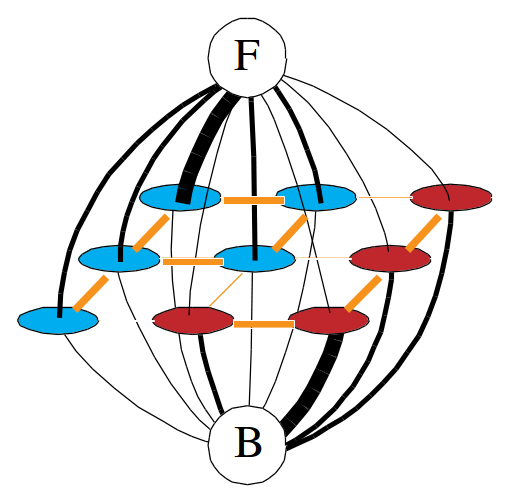
\includegraphics[width=1.2in]{graphcut1.png}
       \end{figure}
       \begin{figure}[!ht]
       \centering
       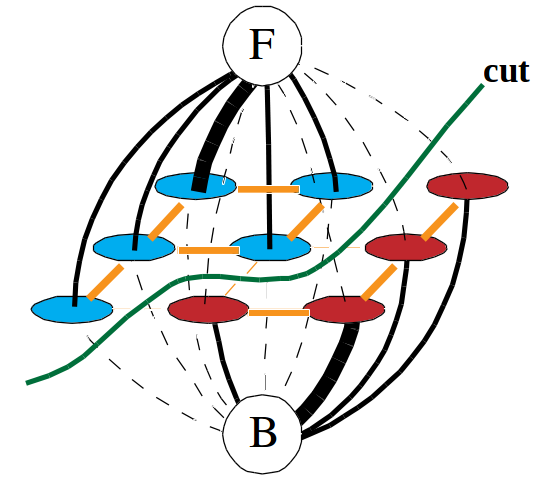
\includegraphics[width=1.2in]{graphcut2.png}
       \end{figure}
      \end{column}
 \end{columns}  
\end{frame}


\begin{frame}
\frametitle{Graph Cuts}
  \begin{figure}[!ht]
  \centering
   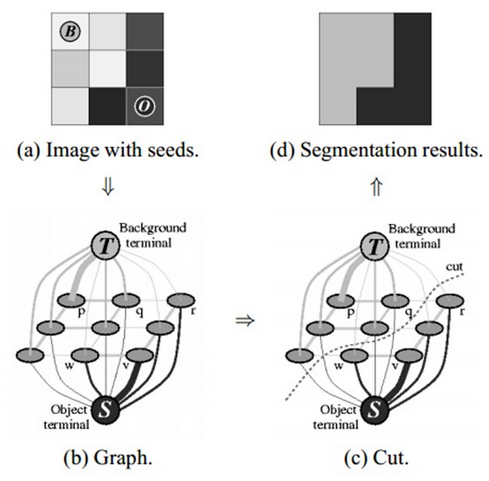
\includegraphics[width=2.2in]{graphcut.png}
   \end{figure}
\end{frame}


\begin{frame}
\frametitle{Graph Cuts}
\begin{columns}
\begin{column}[c]{0.5\textwidth}
       \begin{figure}[!ht]
       \centering
       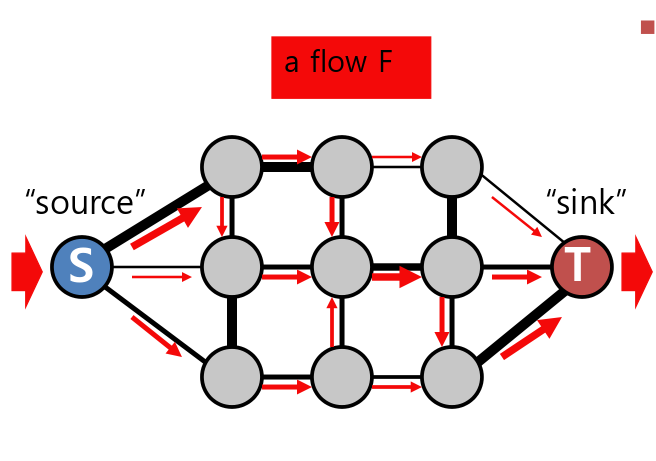
\includegraphics[width=1.9in]{maxflow.png}
       \end{figure}
\end{column}

\begin{column}[c]{0.5\textwidth}
\textbf{Max Flow}:
\begin{itemize}
\item[-] Each edge is a ``{\color{blue} pipe}''
\item[-] Edge {\color{blue} weights} give the pipe's {\color{blue} capacity}
\item[-] S=start  \hspace{0.1in} T=end
\item[-] Find the {\color{blue} largest flow} $F$ of ``water'' that can be sent from ``source'' to ``sink'' along the pipes
\end{itemize}
      \end{column}
 \end{columns}  
\end{frame}



\begin{frame}
\frametitle{Graph Cuts}
%\begin{itemize}
%\item[-] A flow network is defined as a directed graph where an edges has a positive capacity
 A flow in $G$ satisfies the following three properties: $u,v \in V$
	\begin{itemize}
	\item[-] {\color{blue} Capacity Constraint}:  $f(u,v)\leq c(u,v)$ \\
	\item[-] {\color{blue} Skew Symmetry}: $f(u,v) = -f(u,v)$   \\
	\item[-] {\color{blue} Flow Conservation}: $ \sum f(u,v) = 0$ \\
	\end{itemize}
%\end{itemize}
%In graph $G$, the maximum source-to-sink flow possibe is equal to the capacity of the minimum cut in $G$
\end{frame}



\begin{frame}
\frametitle{Graph Cuts}
\begin{columns}
\begin{column}[c]{0.5\textwidth}
       \begin{figure}[!ht]
       \centering
       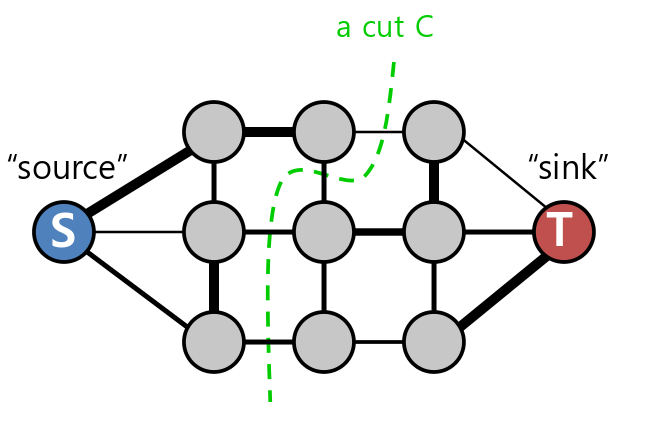
\includegraphics[width=1.9in]{maxflow2.png}
       \end{figure}
\end{column}

\begin{column}[c]{0.5\textwidth}
\textbf{Min Cut}:
\begin{itemize}
\item[-] Find the way to cut the edges so that ``source'' is seperated from ``sink''
\item[-] Cut edges going from source side to sink side
%\item[-] Edge weights now represent cutting cost
\end{itemize}
      \end{column}
 \end{columns}  
\end{frame}




\begin{frame}
\frametitle{Graph Cuts}
\begin{columns}
\begin{column}[c]{0.5\textwidth}
       \begin{figure}[!ht]
       \centering
       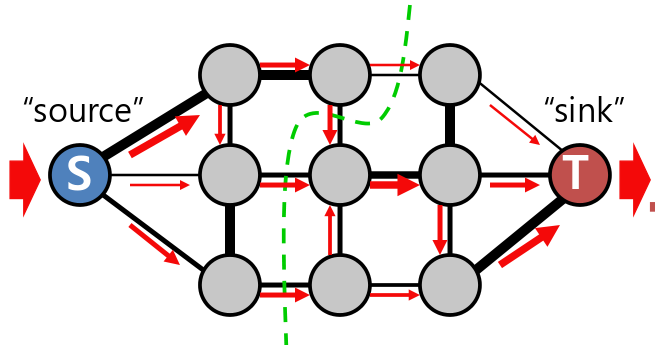
\includegraphics[width=1.9in]{maxflow3.png}
       \end{figure}
\end{column}

\begin{column}[c]{0.5\textwidth}
\textbf{Max Flow = Min Cut}:\\
In graph G, the {\color{blue} maximum source-to-sink flow} possible is equal to the capacity of the {\color{blue} minimum cut} in G.
%\begin{itemize}
%\item[-] Proof sketch: value of a flow is value over any cut
%\item[-] Maximum flow saturates the edges along the munimum cut
%\item[-] Edge weights now represent cutting cost
%\end{itemize}
%Ford and Fulkerson gave first polynomial time algorithm for globally optimal solution 
    \end{column}
 \end{columns}  
\end{frame}





\begin{frame}
\frametitle{Graph Cuts}
    \begin{figure}[!ht]
    \begin{minipage}[t]{0.45\linewidth}
    \centering
    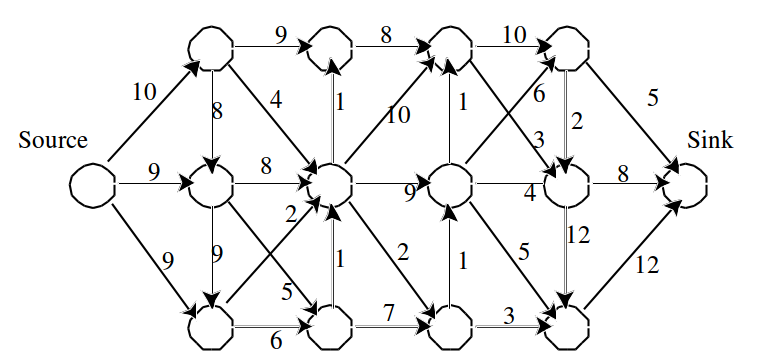
\includegraphics[width=2.2in]{Maxflow1.png}
    \end{minipage}
    \begin{minipage}[t]{0.45\linewidth}
    \centering
    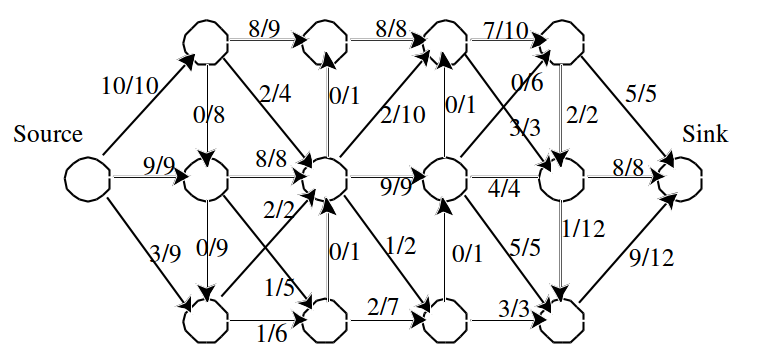
\includegraphics[width=2.2in]{Maxflow2.png}
    \end{minipage}
    \end{figure}
    \begin{figure}[!ht]
    \begin{minipage}[t]{0.45\linewidth}
    \centering
    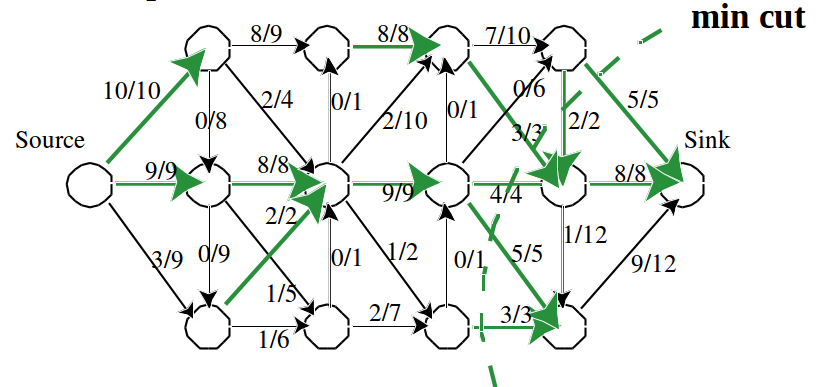
\includegraphics[width=2.2in]{Maxflow3.png}
    \end{minipage}
    \end{figure}
\end{frame}

\begin{frame}
\frametitle{Graph Cuts}
\textbf{Augmenting Path}:
\begin{itemize}
\item[-] Start from zero flow
\item[-] Increase the flow gradually by finding a path from $S$ to $T$, along which more flow can be sent, until a max-flow is achieved
\end{itemize}
  \begin{figure}[!ht]
  \centering
   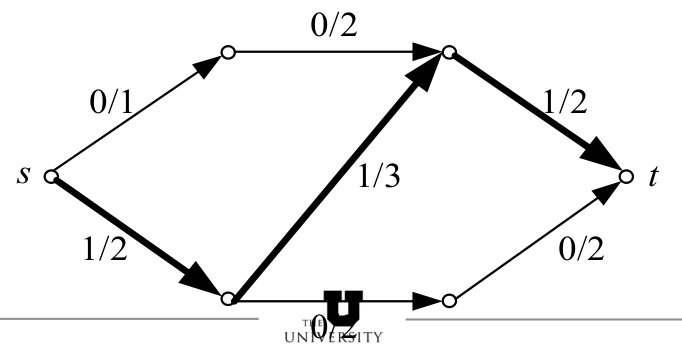
\includegraphics[width=2.2in]{augment.png}
   \end{figure}
\end{frame}

\begin{frame}
\frametitle{Graph Cuts}
  \begin{figure}[!ht]
  \centering
   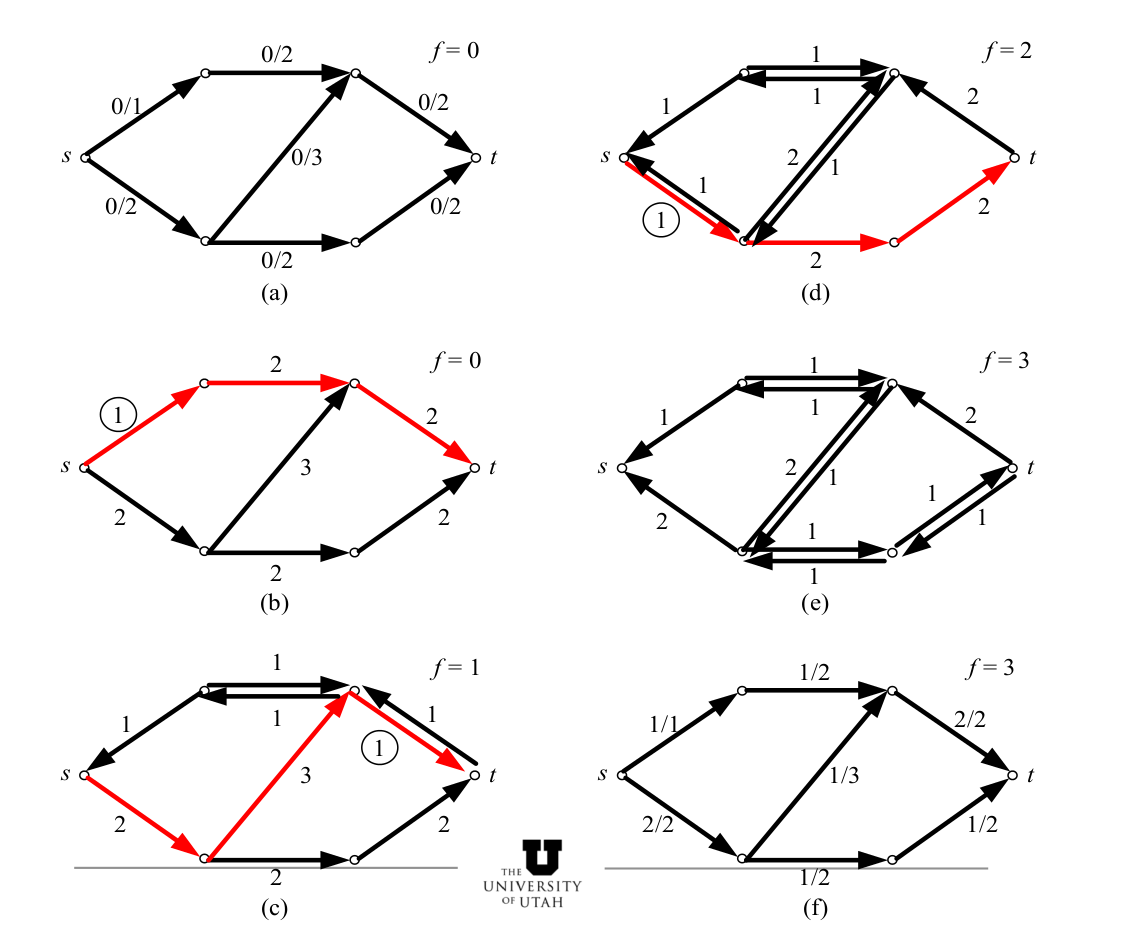
\includegraphics[width=3.4in]{Maxflow4.png}
   \end{figure}
\end{frame}

\begin{comment}
\begin{frame}
\frametitle{Max flow}
\begin{itemize}
\item[-] If $f$ is a flow, then the net flow across the cut ($S$, $T$) is defined to be $f(S,T)$, which is the sum of all edge capacities from $S$ to $T$ subtracted by the sum of all edge capacities from $T$ to $S$
\item[-] The capacity of the cut $(S,T)$ is $c(S,T)$, which is the sum of the capacities of all edge from $S$ to $T$
\item[-] A minimum cut is a cut whose capacity is the minimum over all cuts of $G$
\end{itemize}
\end{frame}
\end{comment}

\section{Grab Cut}
\begin{frame}
\frametitle{Grab Cut}
\textbf{Grab Cut\footnote{``GrabCut Interactive Foreground Extraction using Iterated Graph Cuts'', Carsten Rother. Microsoft Research Cambridge, UK, 2004}}:
\begin{itemize}
\item[-] Uses {\color{blue} GMM} to work with {\color{blue} color images}
\item[-] Alows an {\color{blue} iterative} approach to segmentation
\item[-] Draws {\color{blue} frame} to label possilbe object
\item[-] Adds {\color{blue} Border Matting}
\end{itemize}
\end{frame}


\begin{frame}
\frametitle{Grab Cut}
%\textbf{Iterated Graph Cut}
  \begin{figure}[!ht]
  \centering
   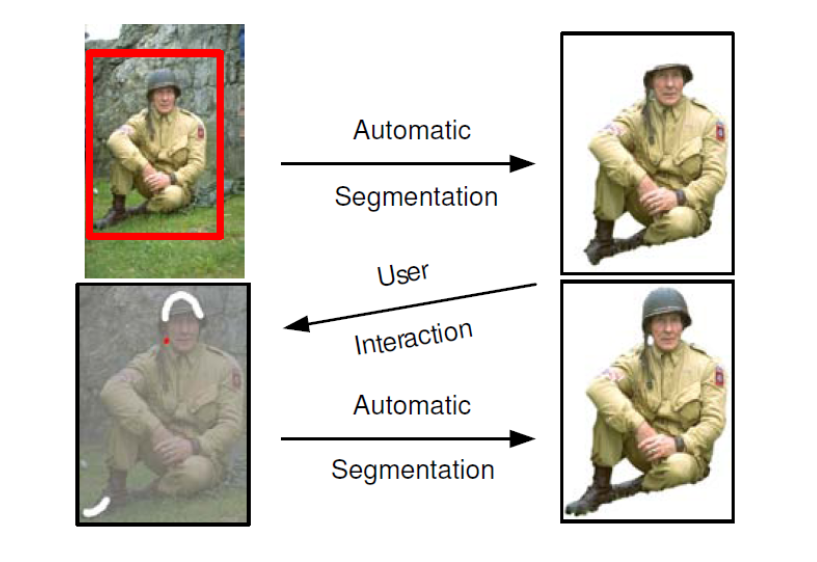
\includegraphics[width=2.2in]{Grab.png}
   \end{figure}
  \begin{figure}[!ht]
  \centering
   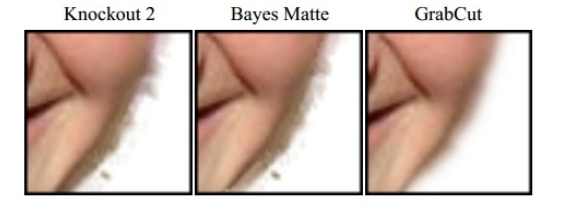
\includegraphics[width=2.2in]{matting.png}
   \end{figure}
\end{frame}

\begin{frame}
\frametitle{Grab Cut}
%\textbf{Iterated Graph Cut}
  \begin{figure}[!ht]
  \centering
   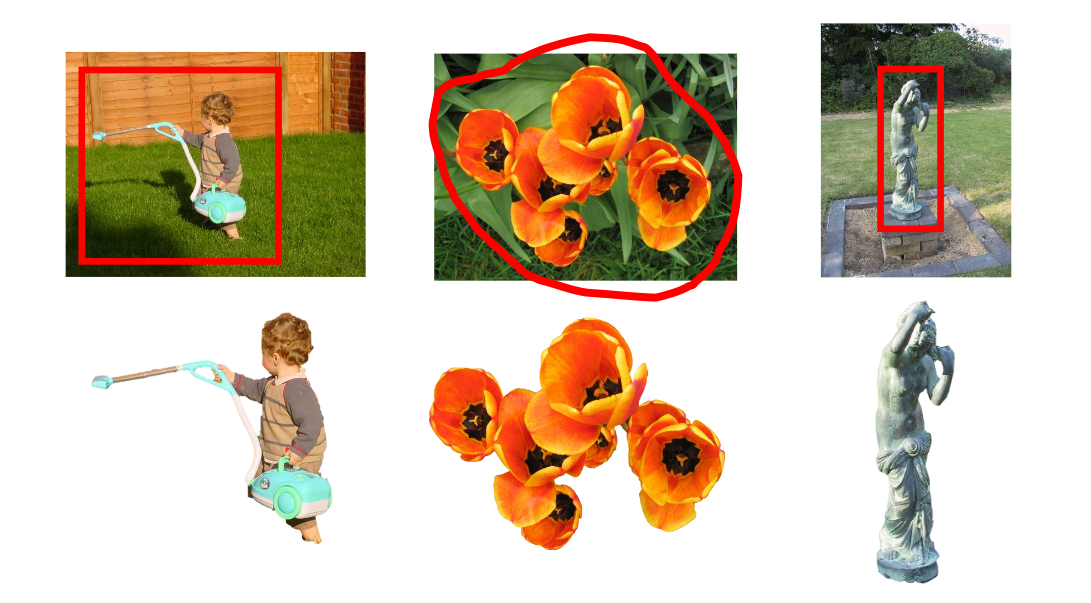
\includegraphics[width=3.0in]{Grab2.png}
   \end{figure}
\end{frame}

\begin{frame}
\frametitle{Graph Cut}
%\textbf{Iterated Graph Cut}
  \begin{figure}[!ht]
  \centering
   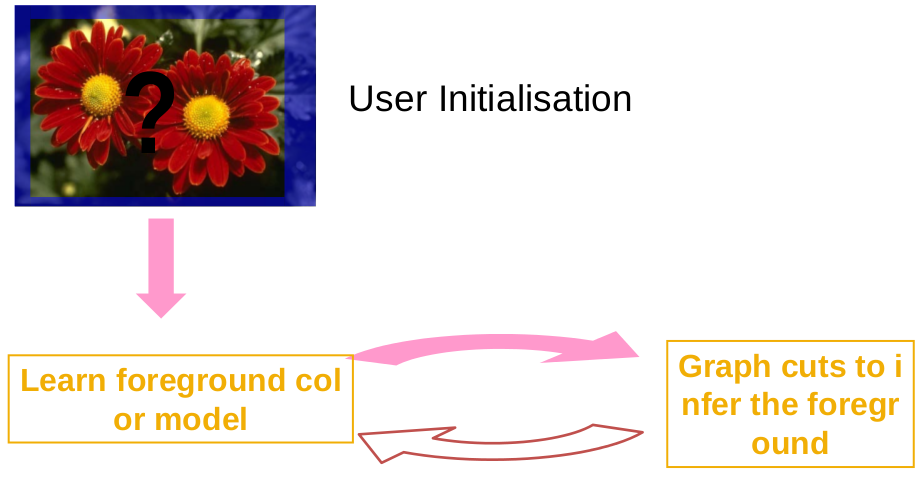
\includegraphics[width=3.0in]{Grab3.png}
   \end{figure}
\end{frame}



\begin{frame}
\frametitle{Grab Cut}
\begin{figure}[!ht]
    \centering
    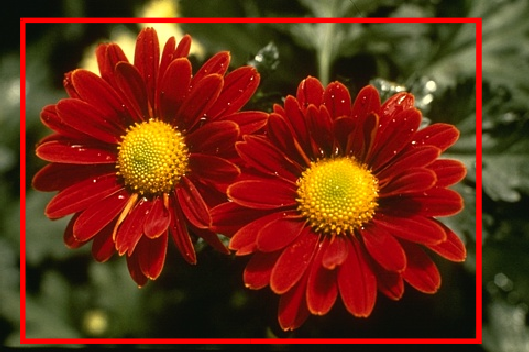
\includegraphics[width=1.8in]{grabcut1.png}
    \end{figure}
    \begin{figure}[!ht]
    \centering
    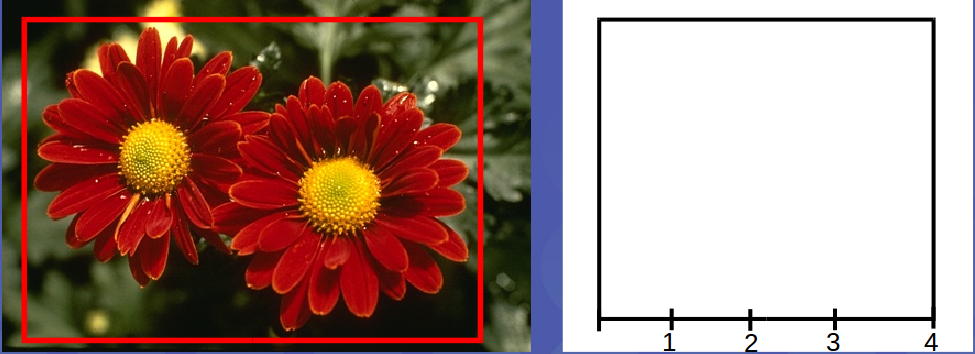
\includegraphics[width=1.8in]{grab1.png}
    \end{figure}
\end{frame}

\begin{frame}
\frametitle{Grab Cut}
    \begin{figure}[!ht]
    \begin{minipage}[t]{0.45\linewidth}
    \centering
    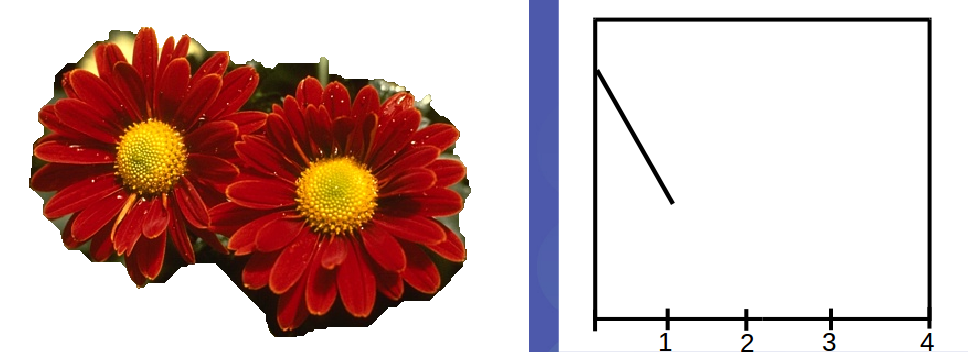
\includegraphics[width=2.0in]{grab2.png}
    \end{minipage}
    \begin{minipage}[t]{0.45\linewidth}
    \centering
    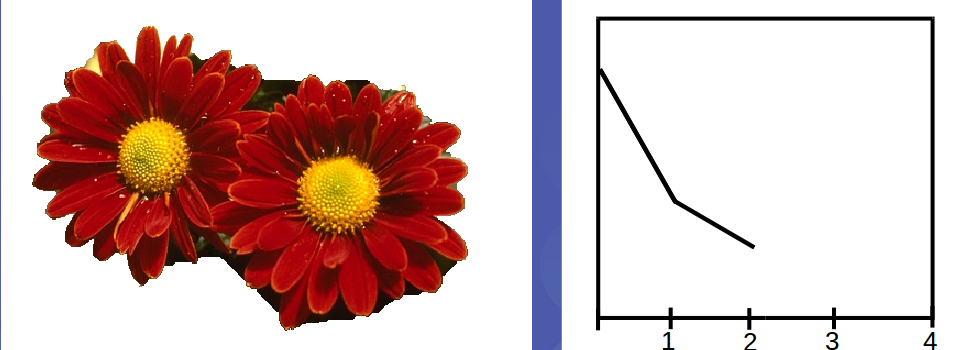
\includegraphics[width=2.0in]{grab3.png}
    \end{minipage}
    \end{figure}
    \begin{figure}[!ht]
    \begin{minipage}[t]{0.45\linewidth}
    \centering
    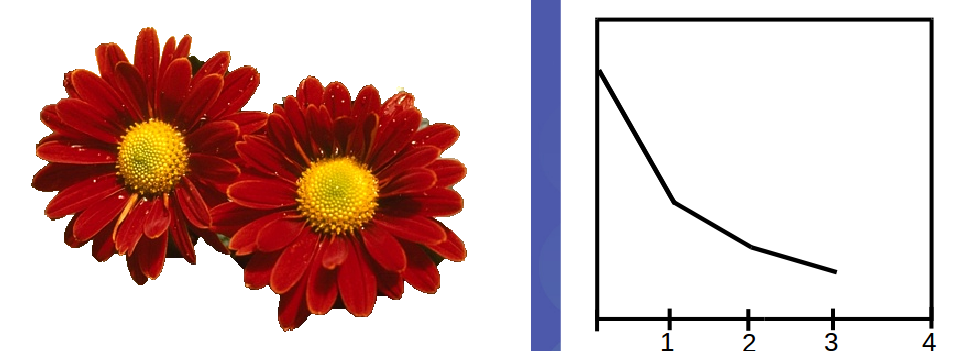
\includegraphics[width=2.0in]{grab4.png}
    \end{minipage}
    \begin{minipage}[t]{0.45\linewidth}
    \centering
    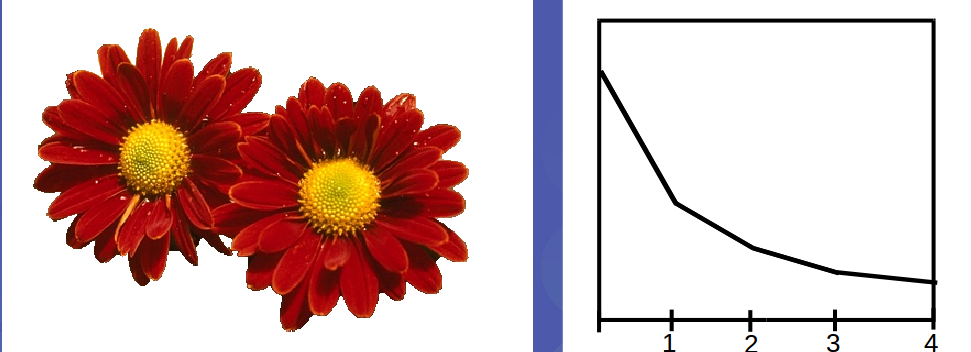
\includegraphics[width=2.0in]{grab5.png}
    \end{minipage}
    \end{figure}
\end{frame}


\begin{frame}
\frametitle{Grab Cut}
\textbf{GMM}: Gaussion Mixture Model\\
\begin{displaymath}
\begin{split}
p(x)=\sum_{k=1}^K p(k)p(x|k) \\
\hspace{0.2in}=\sum_{k=1}^K \pi_k N(x \mid \mu_k, \sigma_k)
\end{split}
\end{displaymath}
\begin{figure}[!ht]
    \centering
    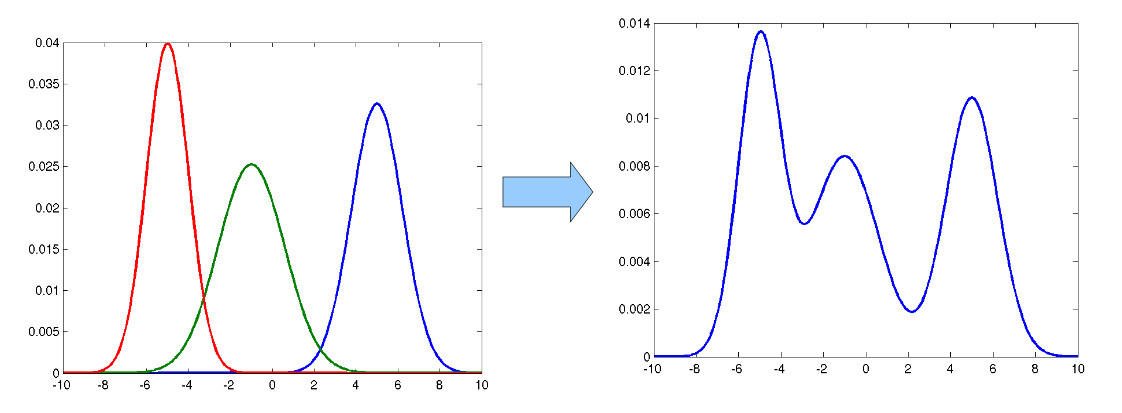
\includegraphics[width=3.0in]{GMM}
\end{figure}
\end{frame}

\begin{frame}
\frametitle{Grab Cut}
\begin{displaymath}
N(x \mid \mu, \Sigma)= \frac{1}{(2\pi)^{D/2}}\frac{1}{\mid \Sigma \mid^{\frac{1}{2}}}\exp(-\frac{1}{2}(x-\mu)^T \Sigma^{-1} (x-\mu))
\end{displaymath}
\begin{figure}[!ht]
    \centering
    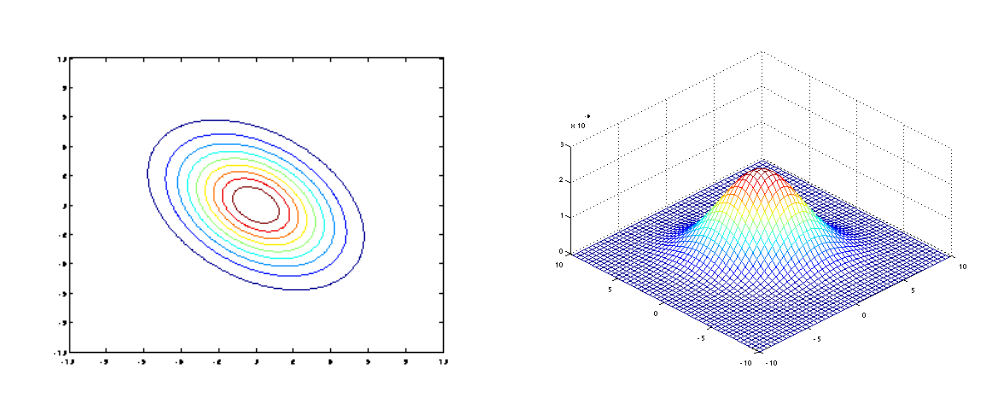
\includegraphics[width=3.0in]{GMM1}
\end{figure}
\end{frame}

\begin{frame}
\frametitle{Grab Cut}
  \begin{figure}[!ht]
  \centering
   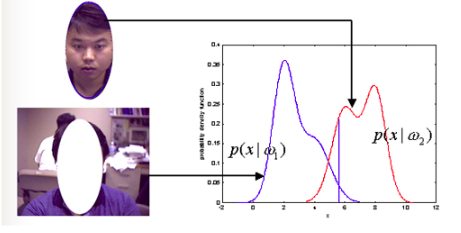
\includegraphics[width=3.0in]{GMM2.png}
   \end{figure}
\end{frame}

\begin{frame}
\frametitle{Grab Cut}
\textbf{Gibbs Energy}:
\begin{flalign*} 
& E(\underline{\alpha}, k, \underline{\theta}, z)=U(\underline{\alpha}, k, \underline{\theta}, z)+V(\underline{\alpha},z) & \\
& &\\
& U(\underline{\alpha}, k, \underline{\theta}, z)=\sum_{n} D(\alpha_{n}, k_{n}, \underline{\theta}, z_{n}) &\\
& D(\alpha_{n}, k_{n}, \underline{\theta}, z_{n})=-\log \pi (\alpha_n,k_{n})+\frac{1}{2} \log \det \Sigma (\alpha_{n},k_{n}) & \\
& +\frac{1}{2}[z_{n}-\mu (\alpha_n,k_{n})]^T \Sigma (\alpha_n,k_{n})^{-1} [z_{n}-\mu (\alpha_n,k_{n})] &\\
& &\\
& \underline{\theta}=\{ \pi (\alpha, k), \mu (\alpha, k), \Sigma (\alpha, k), \hspace{0.1in}\alpha=0,1 \hspace{0.1in}k=1\ldots K\} &\\
& V(\underline{\alpha},z))= \gamma \sum_{(n,n) \in C} [\alpha_{n} \ne \alpha_{m} ]\exp - \beta \parallel z_{m}-z_{n}\parallel^2 &\\
\end{flalign*}
\end{frame}


\begin{frame}
\frametitle{Grab Cut}
\begin{flalign*} 
& U(\underline{\alpha}, k, \underline{\theta}, z)=\sum_{n} D(\alpha_{n}, k_{n}, \underline{\theta}, z_{n}) &
\end{flalign*}
\begin{itemize}
\item[-] $U(\underline{\alpha}, k, \underline{\theta}, z)$ defines {\color{blue} penalty} for {\color{blue} assigning} pixel to object or background
\end{itemize}
\begin{flalign*} 
& D(x)=\sum_{i=1}^{K} \pi_{i} g_{i} (x \mid \mu_{i},\Sigma_{i}),   \hspace{0.2in} \sum_{i=1}^{K} \pi_i =1 &\\
& g(x \mid \mu, \Sigma) = \frac{1}{[(2\pi)^d \mid \Sigma \mid)]^\frac{1}{2}} \exp[-\frac{1}{2} (x-\mu)^T \Sigma^{-1} (x-\mu)]
\end{flalign*}
\begin{itemize}
\item[-] $\mu$, $\Sigma$, $\pi_{i}$ parameters need to learn to define.
\end{itemize}
\end{frame}


\begin{frame}
\frametitle{Grab Cut}
\begin{flalign*} 
& V(\underline{\alpha},z)= \gamma \sum_{(n,n) \in C} [\alpha_{n} \ne \alpha_{m} ]\exp - \beta \parallel z_{m}-z_{n}\parallel^2 &
\end{flalign*}
\begin{itemize}
\item[-] $V(\underline{\alpha},z)$ sets {\color{blue} penalty} of {\color{blue} discontinuities} between pixels of similar intensities
\item[-] $\beta$ is detemined by the contrast to modify the value of $\parallel z_{m}-z_{n}\parallel$
\end{itemize}
\end{frame}


\begin{frame}
\frametitle{Grab Cut}
\textbf{Initialisation}:
\begin{itemize}
\item[step1]  User initialises trimap $T$. The foreground is set to $T_{F}$=1, the background is set to $T_{B}$=0.
\item[step2]  Initialise $\alpha_{n}=0$ for $n \in T_{B}$ and $\alpha_{n}=1$ for $n \in T_{F}$.
\item[step3]  Background and foreground $GMMs$ are initialised from sets $\alpha_{n}=0$ and $\alpha_{n}=1$ respectively.
\end{itemize}
\end{frame}

\begin{frame}
\frametitle{Grab Cut}
\textbf{Iterative minimisation}:
\begin{itemize}
\item[step1] Assign $GMM$ components to pixels: for each $n$ in $T_{F}$:
\begin{displaymath} k_{n}=\arg \min_{k_{n}} D_{n} (\alpha_{n}, k_{n}, \theta, z_{n})\end{displaymath}
\item[step2] Learn $GMM$ parameters from data $z$:
\begin{displaymath} \underline{\theta}=\arg \min_{\underline{\theta}}U({\underline{\alpha}}, k, \underline{\theta}, z) \end{displaymath}
\item[step3] Estimate segmentation: use min cut to solve:
\begin{displaymath} \min_{\{ \alpha_{n}:n \in T_{U}\}}= \min_{k} E(\underline{\alpha}, k, \underline{\theta}, z)  \end{displaymath}
\item[step4] Repeat from $Step 1$, until convergence.
\item[step5] Apply border matting.
\end{itemize}
\end{frame}

\begin{frame}
\frametitle{Grab Cut}
{\color{blue} [Demo]}\\
\textbf{User editing}:
\begin{itemize}
\item[-] \emph{Edit}: fix some pixels either to $\alpha_{n}=0$ (background brush) or $\alpha_{n}=1$ (foreground brush); update trimap $T$ accordingly. Perform $Step 3$ above, just once.
\item[-] \emph{Refine operation}: [optional] perform entire iterative minimisation algorithm .
\end{itemize}
\end{frame}

   

\end{document}
